\documentclass[UTF8]{ctexbook}
\usepackage{graphicx}
\usepackage{amsmath}

\title{桥梁大作业报告}
\author{组长:贺琪 \\ 组员:陈煜 \ 刘畅武 \ 杨昊光 \ 朱子霖}

\begin{document}
\maketitle 

\tableofcontents

%-------------------------这里是这个项目的整体描述---------------------------------
%----------------------------------------------------------------------------------
\newpage
\section{总述}
\subsection{项目描述}
桥模型由桥墩(pier),桥面(floor),支撑梁(support beam),河堤(river bank)和钢缆(cables)五部分组成,其中桥墩和河堤用实体单元建模,桥面用板单元建模,支撑梁用梁单元建模,钢缆用杆单元建模,如图1 所示。\\

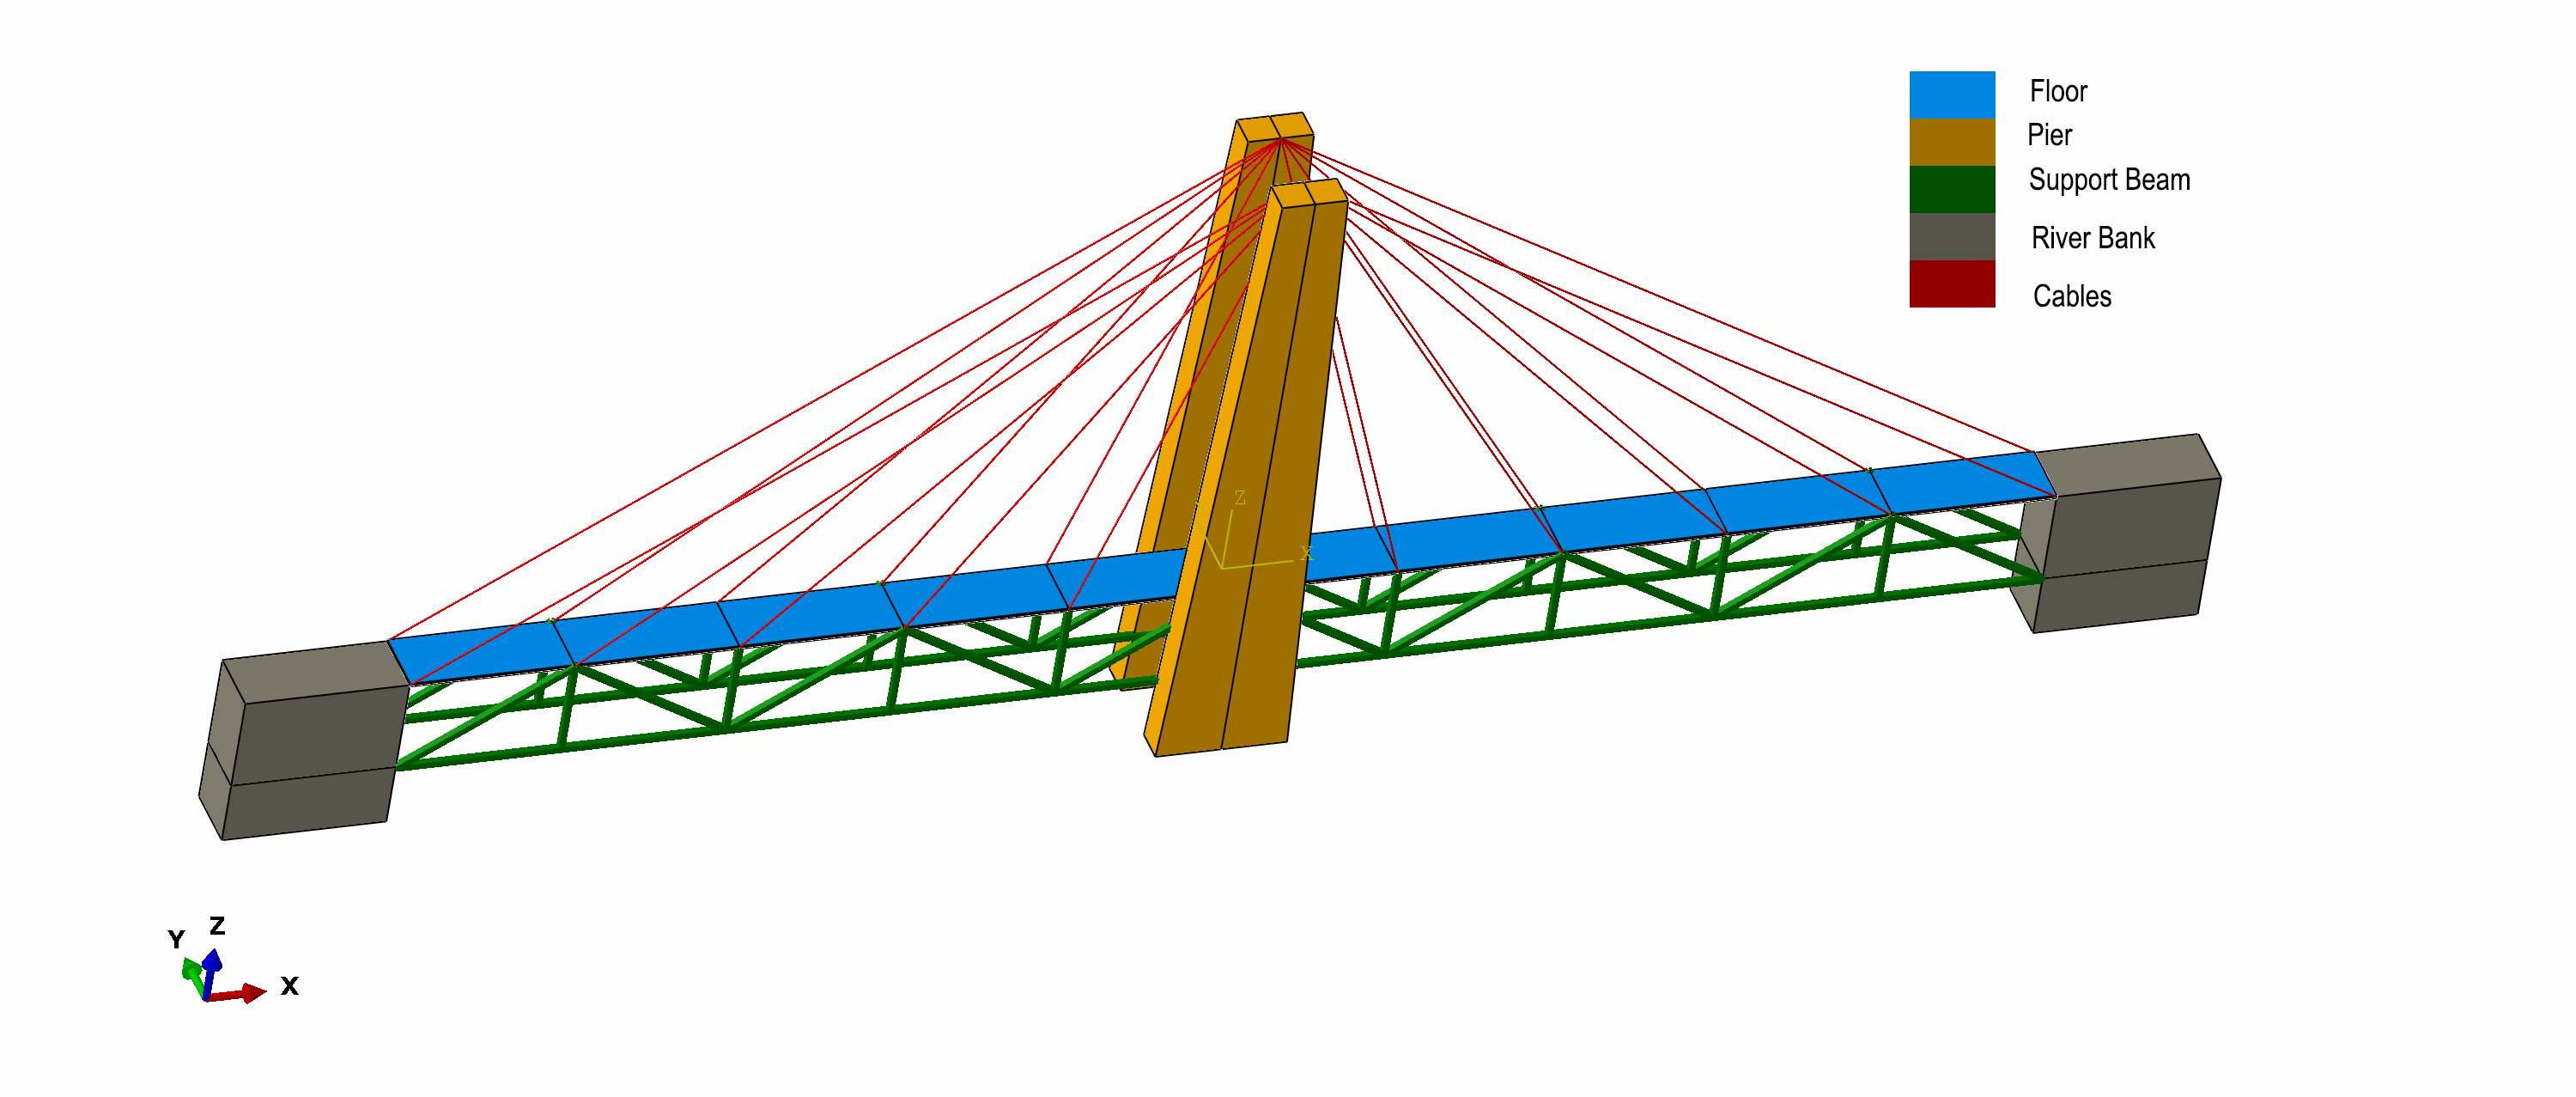
\includegraphics[width=\textwidth]{01.png} % Include the image placeholder.png

\textbf{桥墩}:

桥墩在XZ方向为左右对称梯形,如图2所示,梯形高200,上底为20,下底40,在y方向上厚度为10。桥面位于距桥墩底50处。两个桥墩顶面内侧中点为所有钢缆的与桥墩的连接点。(参照图1)

采用实体单元建模

\begin{center}
\begin{tabular}{ll}
材料&:Concrete\\
弹性模量&:25e9\\
泊松比&:0.3\\
密度&:2320\\
\end{tabular}
\end{center}


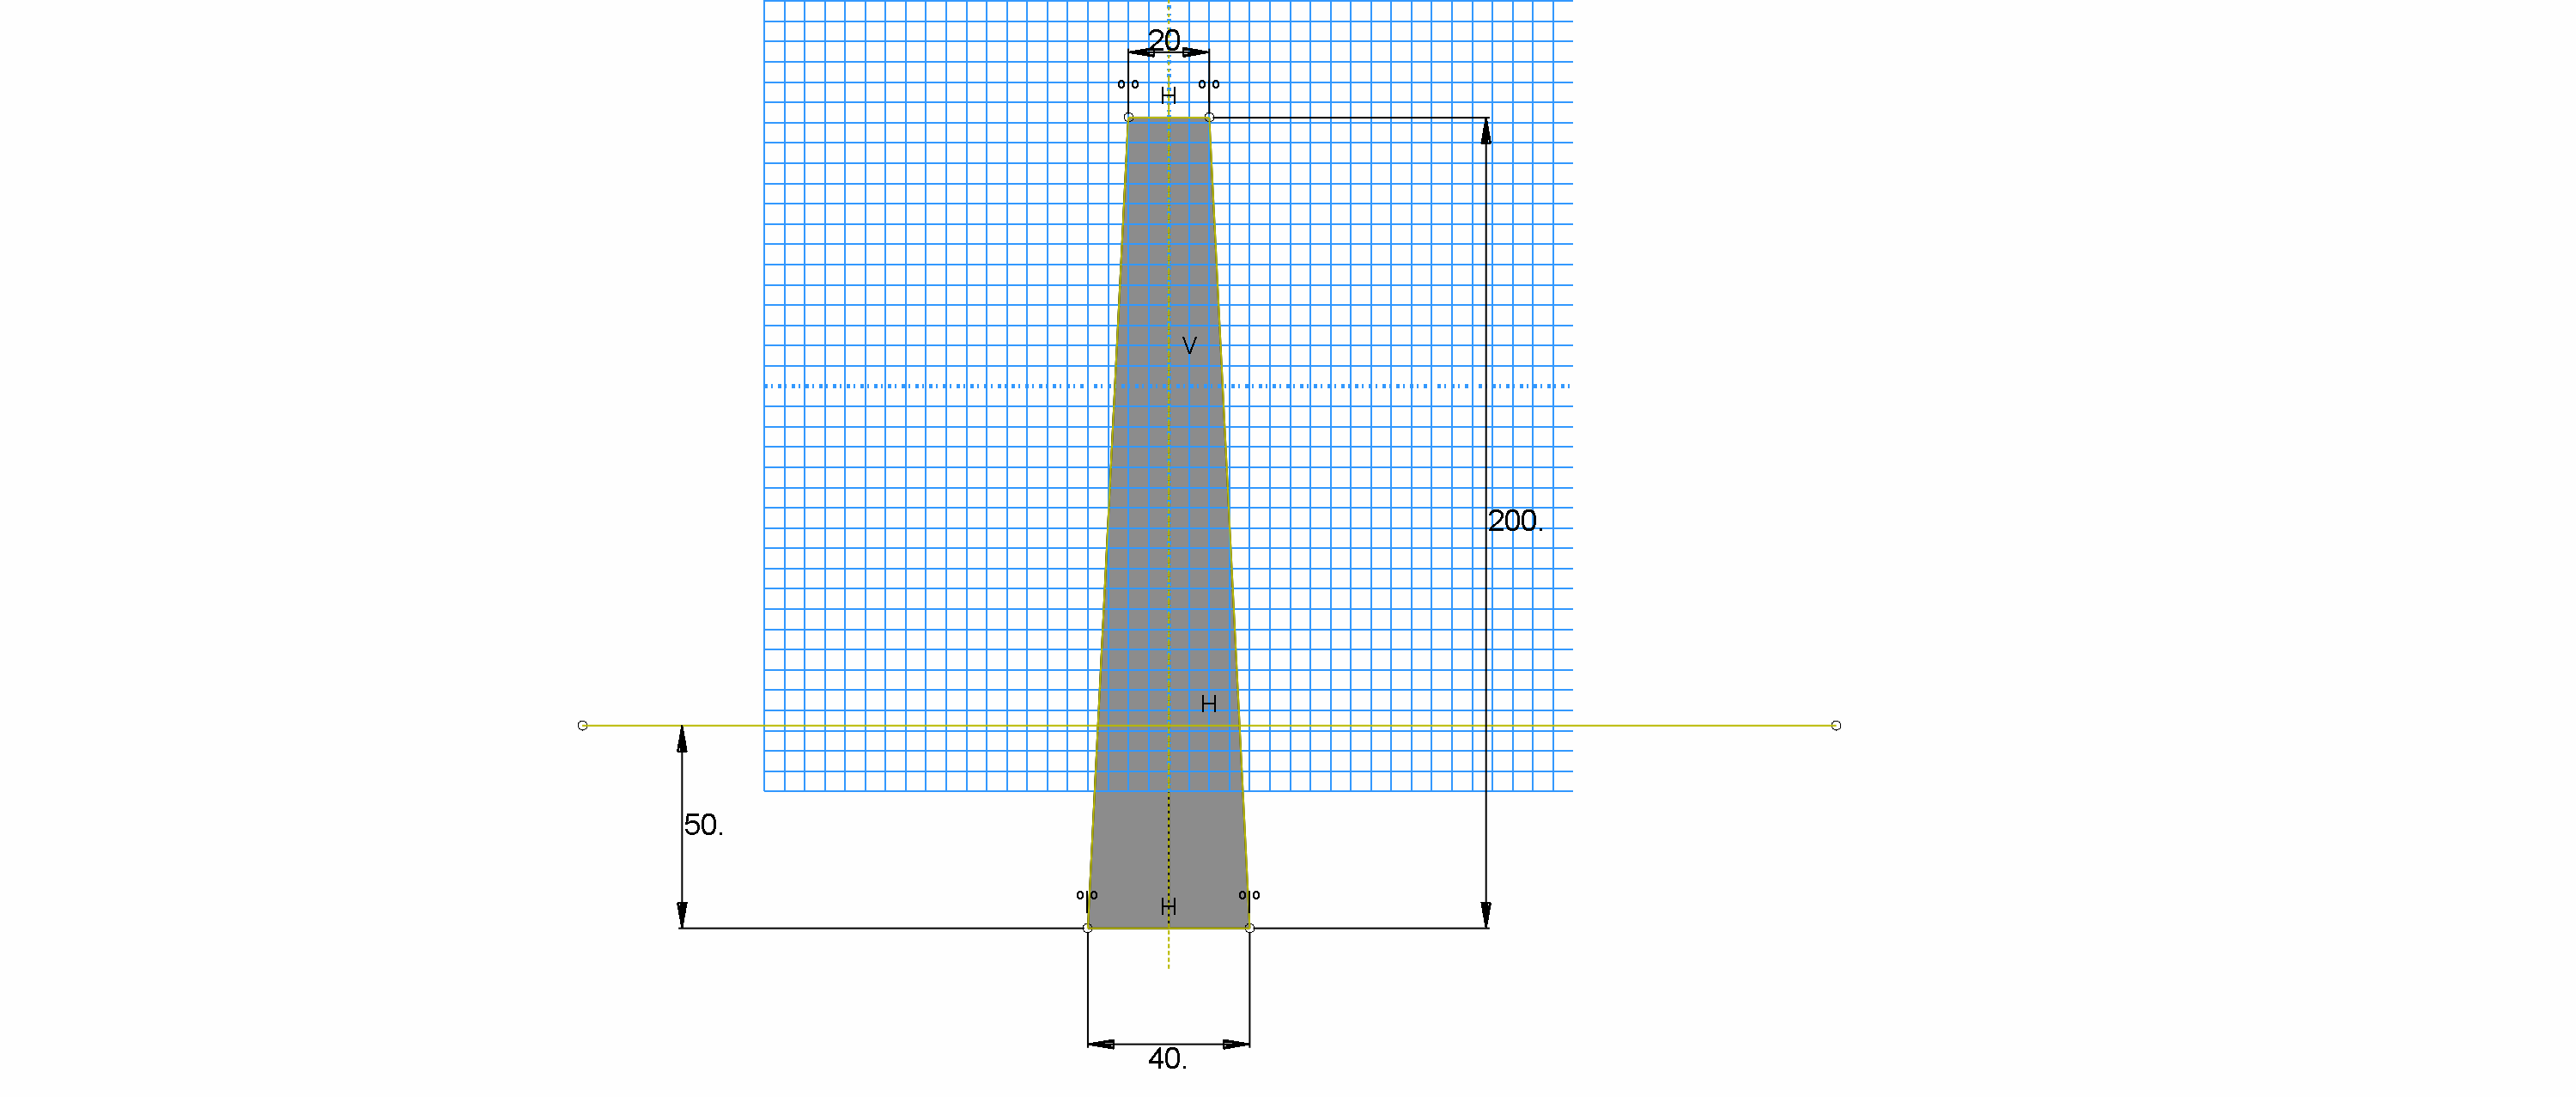
\includegraphics[width=\textwidth]{02.png}

\textbf{桥面}:

桥面位于z=0的平面内,如图3所示,为长方形,长为500,宽为20,厚度为1。在桥面上下边对称地布置钢缆连接点,每个钢缆连接点相距50,共计2×2×5=20个钢缆连接点。每根钢缆另一端连接桥墩顶面内侧中点。(参照图1)

采用板单元建模

\begin{center}
\begin{tabular}{ll}
材料&:Concrete\\
弹性模量&:25e9\\
泊松比&:0.3\\
密度&:2320\\
\end{tabular}
\end{center}

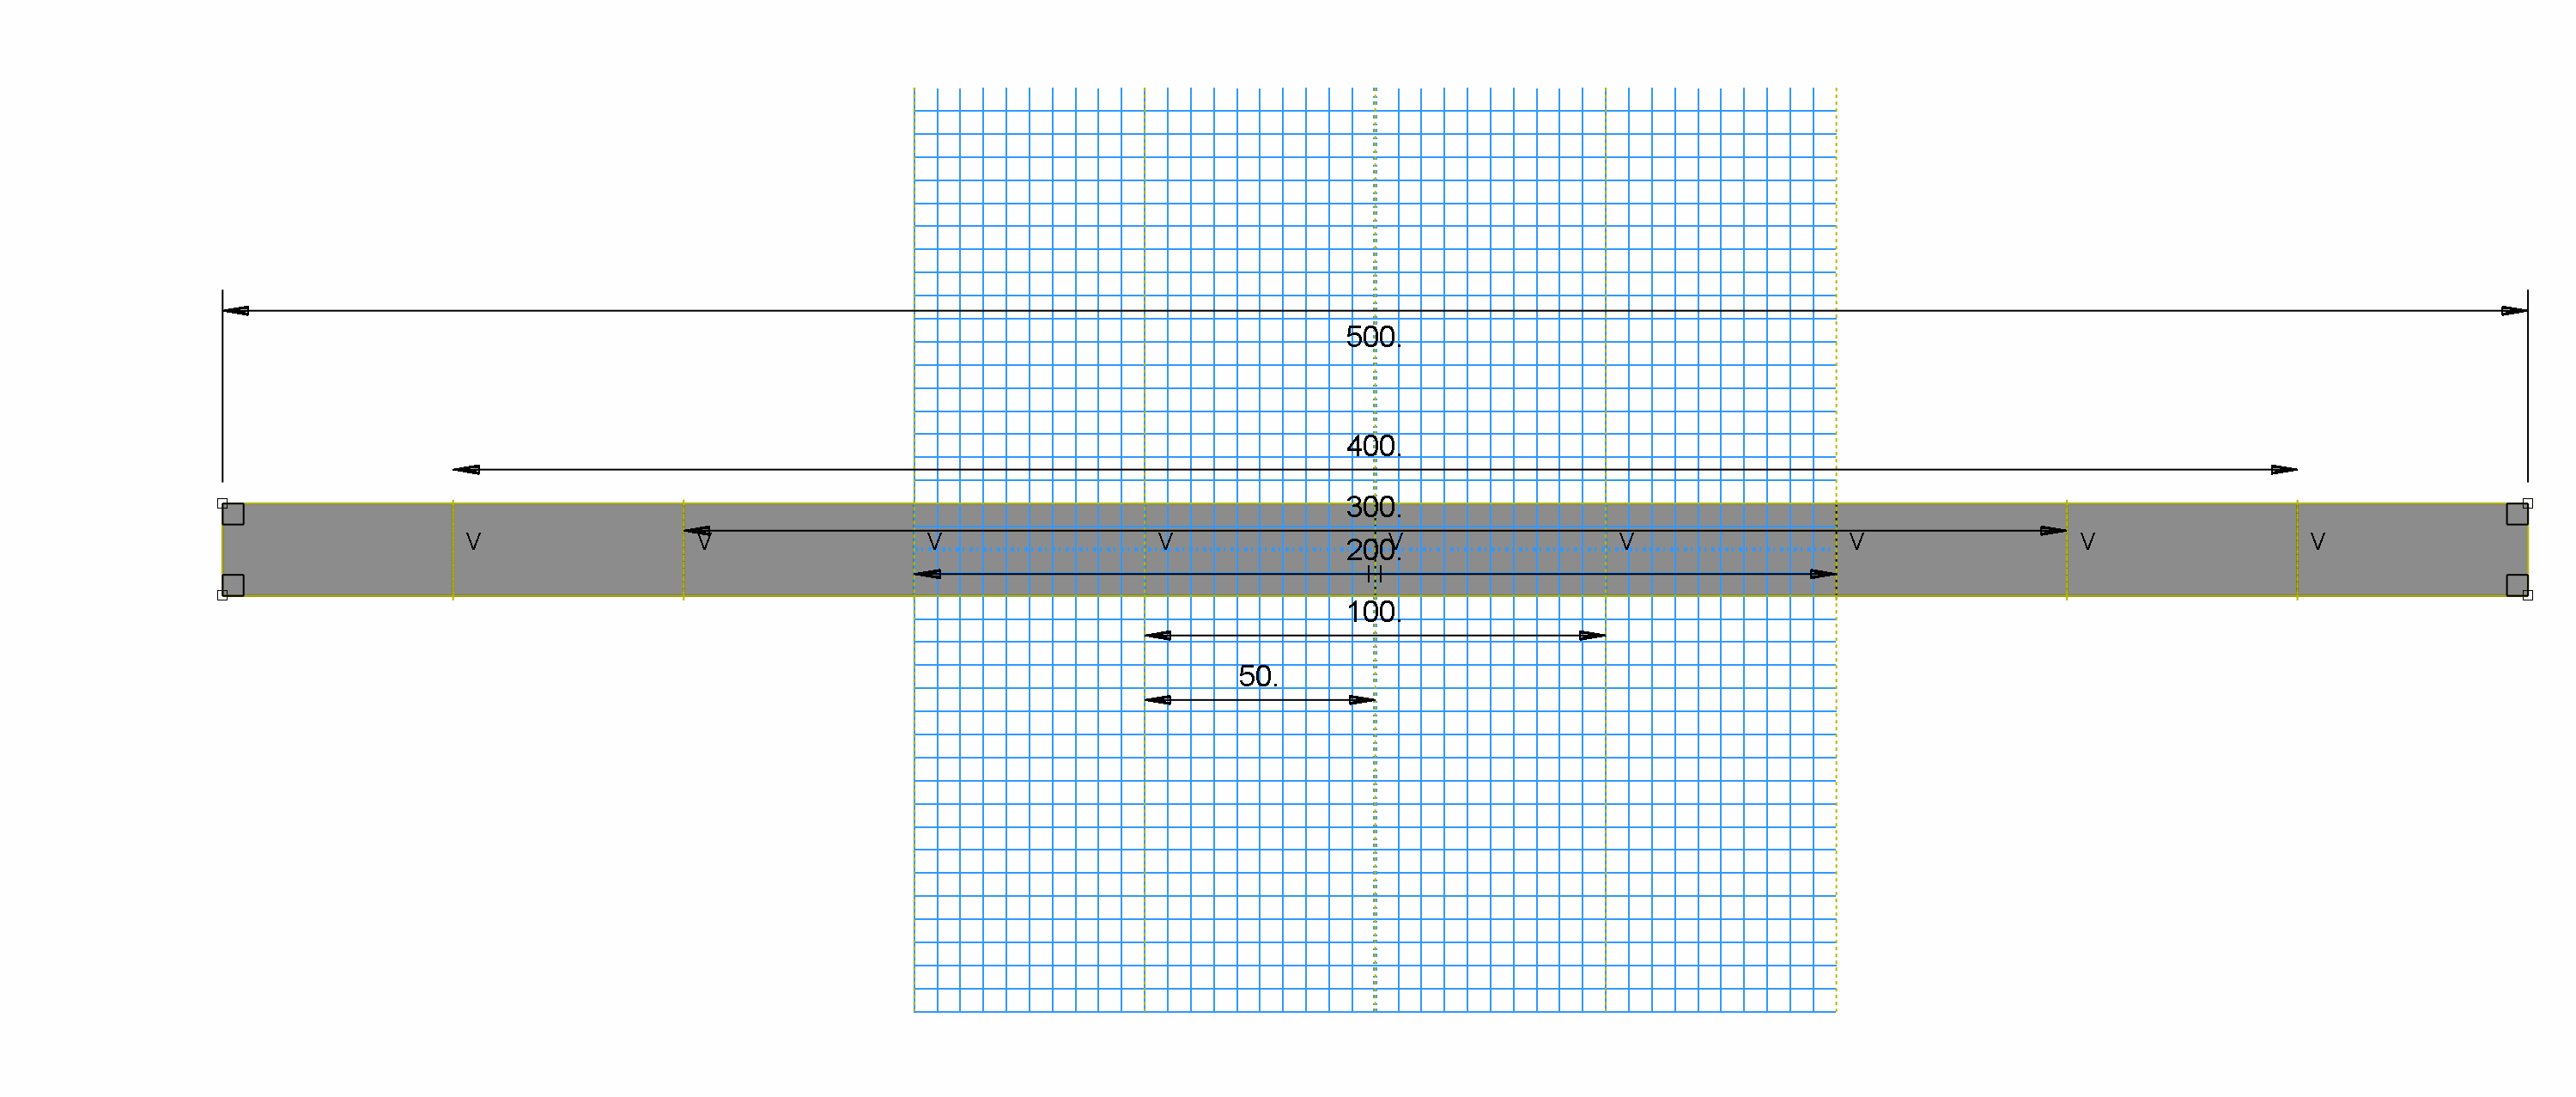
\includegraphics[width=\textwidth]{03.png}

\textbf{河堤}:

河堤为50×50×20的立方体,如图1所示,变长为20的一边与桥面相铰接,另外在距离底面20处与支撑梁相铰接。(铰接指对应结点平动自由度相同,转动自由度自由)

采用实体单元建模。

\begin{center}
\begin{tabular}{ll}
材料&:Granite\\
弹性模量&:60e9\\
泊松比&:0.27\\
密度&:2770\\
\end{tabular}
\end{center}

\textbf{支撑梁}:

支撑梁共有两组,分别位于桥面两侧下方,其结构左右对称,如图4所示。支撑梁上部每个结点与桥面相铰接,两组共计2×9=18个结点。两端结点与河堤相铰接,共计2×2=4个结点。

采用梁单元建模,梁截面为正方形筒,边长为2,厚度为0.1。

\begin{center}
\begin{tabular}{ll}
材料&:Aluminum\\
弹性模量&:70e9\\
泊松比&:0.346\\
密度&:2710\\
\end{tabular}
\end{center}

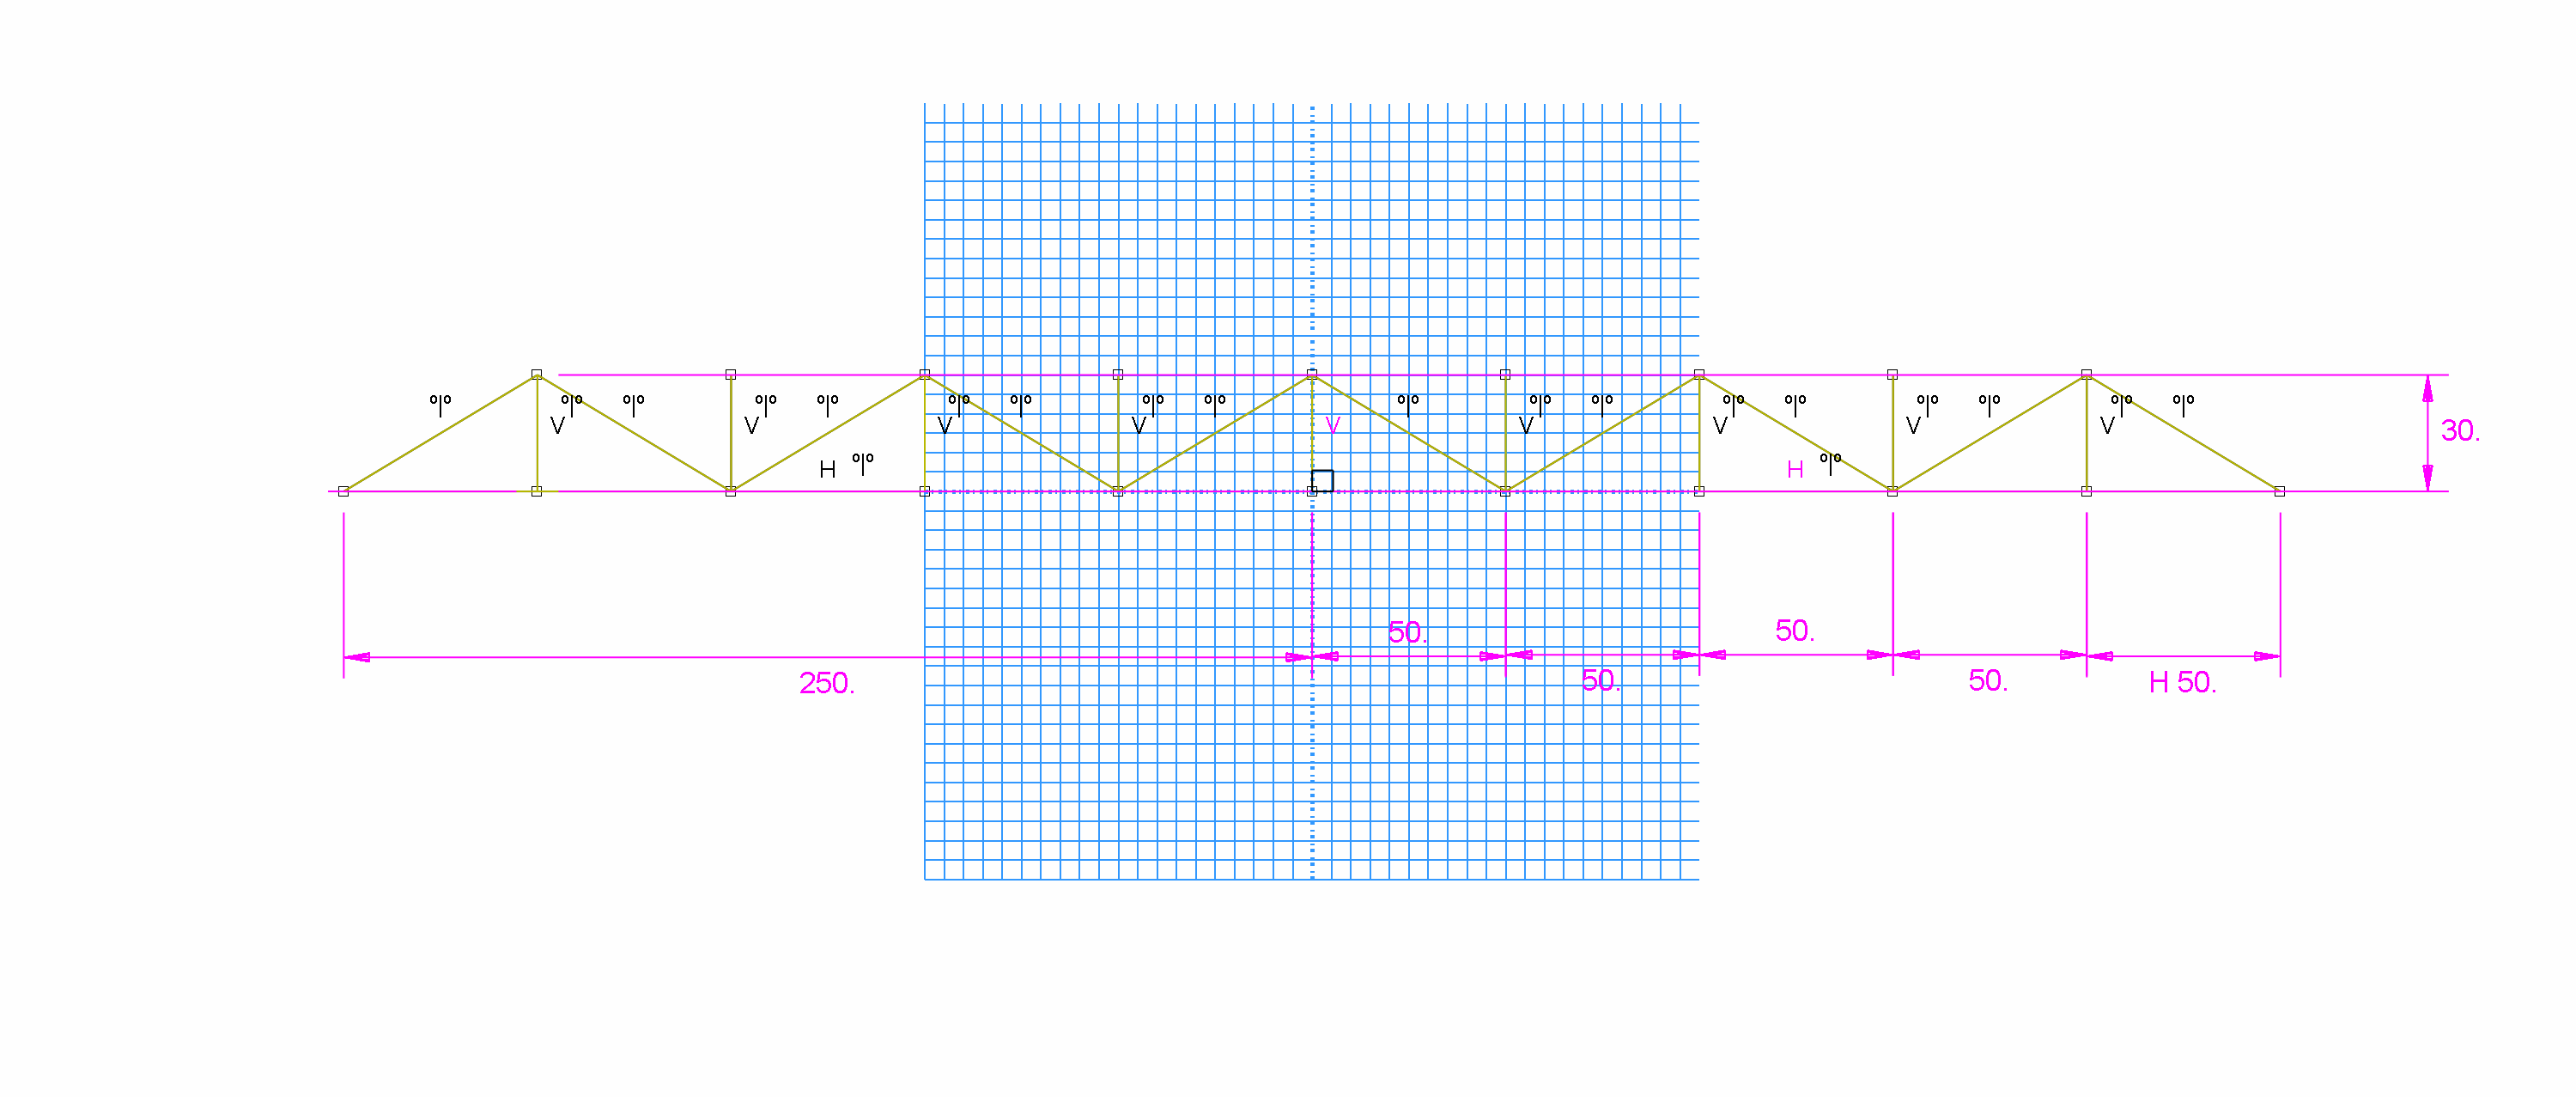
\includegraphics[width=\textwidth]{04.png}

\textbf{钢缆}:

连接桥面与桥墩,共计2×2×5=20根。每根截面积为0.25。

采用杆单元建模

\begin{center}
\begin{tabular}{ll}
材料&:Steel\\
弹性模量&:117e9\\
泊松比&:0.266\\
密度&:7860\\
\end{tabular}
\end{center}

\subsection{Abaqus结果}
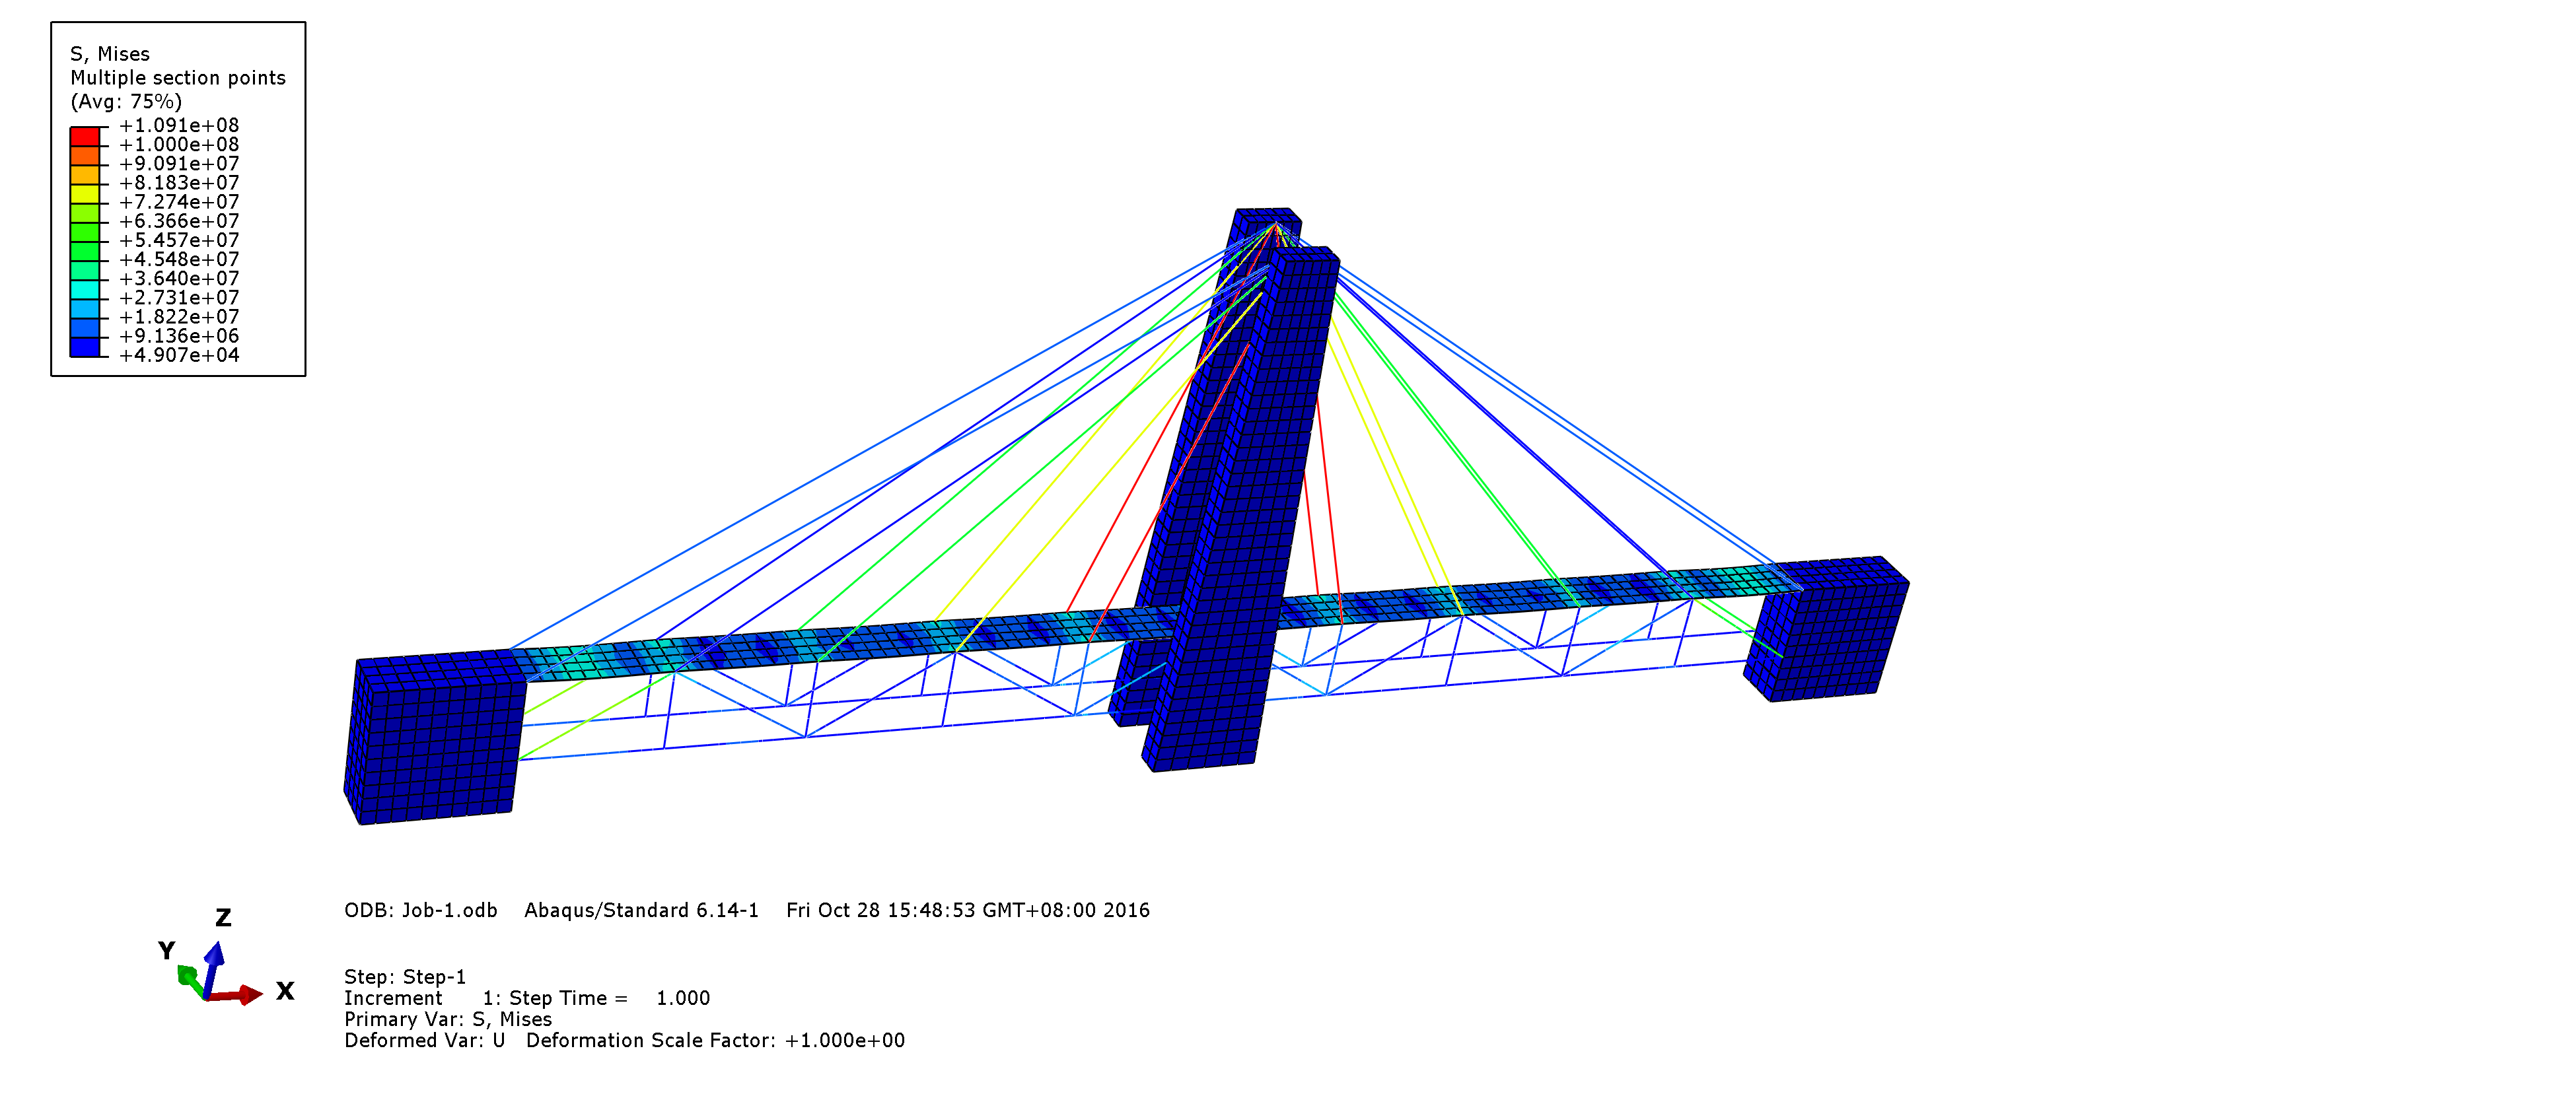
\includegraphics[width=\textwidth]{05.png}


%-------------------------这里是各个部分的描述-------------------------------------
%----------------------------------------------------------------------------------
\section{桥梁功能实现方案}
\subsection{前处理}

%-----------------------------------------------------SPR----------------------------------------------%
\subsection{SPR}

采用SPR方法进行节点应力恢复。对于一个内部节点,若与8个8H单元相连,则有$n=8\times8=64$个高斯点用于应力恢复;对于一个边界面上的节点,则与4个单元相连,有32个高斯点用于应力恢复;同理,对于边界棱上的节点有16个,边界顶点上的节点有8个高斯点。为防止过拟合,对于边界面上的节点和内部节点采用完备二阶多项式进行最小二乘逼近,对于边界棱和边界顶点上的节点采用完备一阶多项式进行最小二乘逼近。以三维单元为例:
\begin{itemize}
\item 对二阶逼近:


\[
\boldsymbol{A}=\begin{bmatrix}1 & x_{1} & y_{1} & z_{1} & x_{1}y_{1} & y_{1}z_{1} & z_{1}x_{1}\\
1 & x_{2} & y_{2} & z_{2} & x_{2}y_{2} & y_{2}z_{2} & z_{2}x_{2}\\
\vdots & \vdots & \vdots & \vdots & \vdots & \vdots & \vdots\\
1 & x_{n} & y_{n} & z_{n} & x_{n}y_{n} & y_{n}z_{n} & z_{n}x_{n}
\end{bmatrix},\ \boldsymbol{X}=\begin{bmatrix}1 & x & y & z & xy & yz & zx\end{bmatrix}
\]



\[
\boldsymbol{C}_{ij}=\begin{bmatrix}c_{0} & c_{1} & c_{2} & c_{3} & c_{4} & c_{5} & c_{6}\end{bmatrix}^{T},\ \boldsymbol{S}_{ij}=\begin{bmatrix}\sigma_{ij}^{(1)} & \sigma_{ij}^{(2)} & \cdots & \sigma_{ij}^{(n)}\end{bmatrix}^{T}
\]



最小二乘逼近为解系数矩阵$\boldsymbol{C}_{ij}$,使得:$\boldsymbol{AC}_{ij}=\boldsymbol{S}_{ij},\ \text{即}\boldsymbol{A}^{T}\boldsymbol{AC}_{ij}=\boldsymbol{A}^{T}\boldsymbol{S}_{ij}$。最后解$\boldsymbol{X}^{(k)}\boldsymbol{C}_{ij}=S_{ij}^{(k)}$为第$k$个节点上的应力。

\item 对一阶逼近:


同理,但只取$1,\ x,\ y,\ z$的项使用。

\item 当连接到一个节点的所有单元具有的高斯点都不足以满足系数要求,或单元采用的为直接刚度法时,转而采用节点平均法恢复应力。这种情况常见于梁、杆、3T单元等。
\end{itemize}

\subsection{后处理}

%-------------------------------------------------------8H--------------------------------------------------%
\subsection{8H}
\begin{enumerate}
\item 算法分析

\begin{itemize}
\item 位移计算


给出一个8H单元,其节点坐标矩阵为$\boldsymbol{X}=\begin{bmatrix}x_{1} & y_{1} & z_{1}\\
x_{2} & y_{2} & z_{2}\\
\vdots & \vdots & \vdots\\
x_{8} & y_{8} & z_{8}
\end{bmatrix}$,每条边的方向上采用2点高斯积分,共8个高斯点,并采用三线性函数作为形函数。作前处理时,将坐标变换到$\xi,\ \eta,\ \zeta$下求形函数的梯度,再对8个高斯点作加权求和,得到单元刚度阵:


\[
N_{i}=\frac{1}{8}(1+\xi_{i}\xi)(1+\eta_{i}\eta)(1+\zeta_{i}\zeta),\ i=1,2,...,8
\]
\[
\boldsymbol{N}=\begin{bmatrix}\boldsymbol{N}_{1} & \boldsymbol{N}_{2} & \boldsymbol{N}_{3} & \boldsymbol{N}_{4} & \boldsymbol{N}_{5} & \boldsymbol{N}_{6} & \boldsymbol{N}_{7} & \boldsymbol{N}_{8}\end{bmatrix},\ \boldsymbol{N}_{i}=N_{i}\begin{bmatrix}1\\
 & 1\\
 &  & 1
\end{bmatrix}
\]
\[
GN=\begin{bmatrix}\frac{\partial N_{1}}{\partial\xi} & \frac{\partial N_{2}}{\partial\xi} & \cdots & \frac{\partial N_{8}}{\partial\xi}\\
\frac{\partial N_{1}}{\partial\eta} & \frac{\partial N_{2}}{\partial\eta} & \cdots & \frac{\partial N_{8}}{\partial\eta}\\
\frac{\partial N_{1}}{\partial\zeta} & \frac{\partial N_{2}}{\partial\zeta} & \cdots & \frac{\partial N_{8}}{\partial\zeta}
\end{bmatrix}
\]



\[
\boldsymbol{B}=\nabla_{s}\boldsymbol{N}=\begin{bmatrix}\boldsymbol{B}_{1} & \boldsymbol{B}_{2} & \boldsymbol{B}_{3} & \boldsymbol{B}_{4} & \boldsymbol{B}_{5} & \boldsymbol{B}_{6} & \boldsymbol{B}_{7} & \boldsymbol{B}_{8}\end{bmatrix},\ \boldsymbol{B}_{i}=\begin{bmatrix}B_{ix} & 0 & 0\\
0 & B_{iy} & 0\\
0 & 0 & B_{iz}\\
B_{iy} & B_{ix} & 0\\
0 & B_{iz} & B_{iy}\\
B_{iz} & 0 & B_{ix}
\end{bmatrix},\ i=1,2,...,8
\]



$\boldsymbol{B}$矩阵的各量由单元Jacobian矩阵和形函数对各坐标的导数得到:


\[
\boldsymbol{J}^{-1}\cdot GN=\begin{bmatrix}B_{1x} & B_{2x} & \cdots & B_{8x}\\
B_{1y} & B_{2y} & \cdots & B_{8y}\\
B_{1z} & B_{2z} & \cdots & B_{8z}
\end{bmatrix},\ \boldsymbol{J}=GN\cdot\boldsymbol{X}^{T}
\]



$\boldsymbol{D}$矩阵由本构关系得到,在此认为材料是各向同性的:


\[
\sigma_{ij}=2G\varepsilon_{ij}+\lambda\varepsilon_{kk}\delta_{ij}
\]
$\Rightarrow\boldsymbol{D}=\begin{bmatrix}2G+\lambda & \lambda & \lambda\\
\lambda & 2G+\lambda & \lambda\\
\lambda & \lambda & 2G+\lambda\\
 &  &  & 2G\\
 &  &  &  & 2G\\
 &  &  &  &  & 2G
\end{bmatrix},\ \text{s.t. }\boldsymbol{\sigma}=\boldsymbol{D\varepsilon},\ \text{where }\boldsymbol{\varepsilon}=\begin{bmatrix}\varepsilon_{x}\\
\varepsilon_{y}\\
\varepsilon_{z}\\
\varepsilon_{xy}\\
\varepsilon_{yz}\\
\varepsilon_{zx}
\end{bmatrix},\ \boldsymbol{\sigma}=\begin{bmatrix}\sigma_{x}\\
\sigma_{y}\\
\sigma_{z}\\
\tau_{xy}\\
\tau_{yz}\\
\tau_{zx}
\end{bmatrix}$.


\[
\boldsymbol{K}^{e}=\sum_{i=1}^{2}\sum_{j=1}^{2}\sum_{k=1}^{2}w_{i}w_{j}w_{k}\boldsymbol{B}^{T}(\xi_{i},\eta_{j},\zeta_{k})\boldsymbol{DB}(\xi_{i},\eta_{j},\zeta_{k})
\]



生成单元刚度阵通过Location Matrix进行组装,得到全局的刚度阵,再解$\boldsymbol{Kd=f}$.

\item 算法实现


位移计算部分按照变换将坐标变换到$[-1,1]\times[-1,1]\times[-1,1]$后即可得到形函数和各导数。取得高斯点位置,代入$\boldsymbol{D}$矩阵即可以产生单元刚度阵,调用COLHT和ADDBAN生成总刚度矩阵并求解。


SPR部分,在前处理时保存单元连接矩阵到临时文件中,在后处理中调取,计算每个节点连接的单元数量和编号,以及用于恢复节点位置的信息,生成为NodeRelationFlag数组。对每个节点,根据该数组选取逼近的阶次,计算$\boldsymbol{A}\text{、}\boldsymbol{S}$矩阵,并传入最小二乘子程序LeastSquare中,得到系数数组,并代入节点位置信息,得到恢复的节点应力。

\item 算法测试


Patch Test 选取了7单元模型和8单元模型进行测试,测试形状为单位立方体,$E=1000,\ \nu=0.25$,通过内部确定1个或8个点来将其分划为8个或7个单元。施加线性位移场:


\[
u_{x}=0.001x,\ u_{y}=0.002y,\ u_{z}=0.003z
\]



得到各点需要施加的外力,并采用最少的边界条件对单元进行测试。测试结果如 data/8H 中各输入输出文件所示。


测试结果表明,对于线性场,输出误差在机器$\varepsilon$量级,单元设计能精确重构线性位移场,为一阶收敛的。


对SPR的测试,其输出结果误差也在机器$\varepsilon$量级,因而从算法设计的角度来说是合理的。\end{enumerate}

\subsection{Beam}

\subsection{Shell}

\subsection{半带宽优化}

\subsection{稀疏存储求解器}

%-------------------------这里是其他单元的描述-------------------------------------
%----------------------------------------------------------------------------------
\section{其他单元}
\subsection{3T}

\subsection{4Q}

\subsection{6T}

\subsection{8Q}

\subsection{9Q}

\subsection{4T}

\subsection{铁木辛柯梁}

\subsection{Plate}

\subsection{无限单元}

\subsection{超级单元}

\subsection{过渡单元}

%-------------------------这里是其他功能的描述-------------------------------------
%----------------------------------------------------------------------------------
\section{高级功能}
\subsection{弹塑性杆分析}

\subsection{模态分析}

\subsection{动力学响应分析}

\end{document}
